\subsection{Rys historyczny}
\begin{figure}
    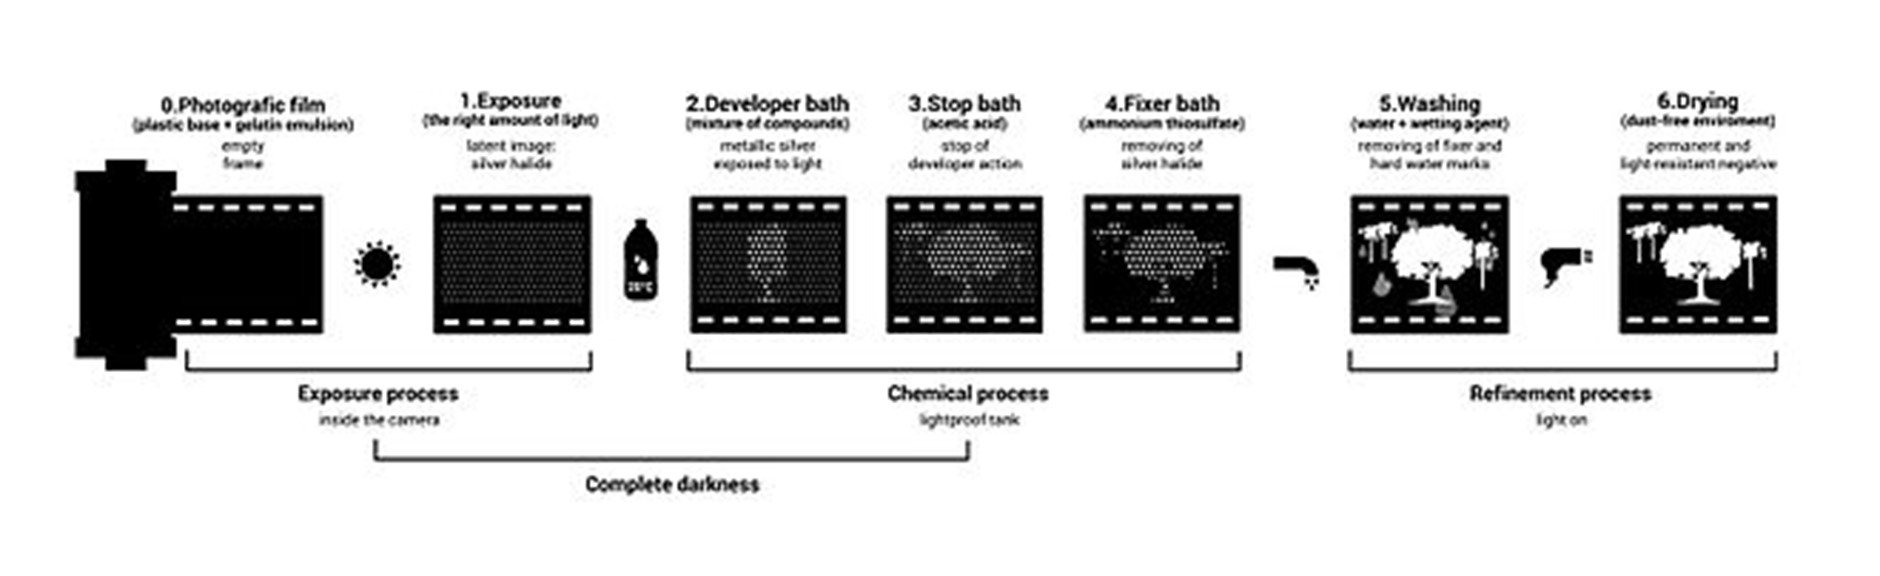
\includegraphics{./images/Picture1.jpg}
    \caption{Wywoływanie biało czarnej kliszy}
    \label{fig:wywolywanie}
\end{figure}
\subsubsection{Wywoływanie zdjęć}
Przetwarzanie obrazów to nie jest technologia, która mogła zacząć istnieć po wynalezieniu komputerów. Używając aparatów korzystających z kliszy filmowej, po ekspozycji należy go poddać procesowi wywoływania. Polega on na wyciągnięciu pierwotnego efektu naświetlenia do obrazu, który oddaje scenę uchwyconą przez aparat. \cite{doi:https://doi.org/10.1002/14356007.a20_001} Proces w przypadku zdjęć aparatem na kliszę polega na zanurzaniu jej w odpowiednich związkach chemicznych na określone ilości czasu by otrzymać zamierzony efekt. 

Istnieją wariacje na temat takiego przetwarzania, różni się ono trochę w zależności od technologii kliszy. W niektórych przypadkach należy wywołać pozytyw zamiast negatywu. \cite{almanac} Następnie po wywoływaniu można poddać obróbce dalszymi chemikaliami jak np. siarczek sodu dla uzyskania efektu sepii. \cite{sepia} 

\subsubsection{Cyfrowe przetwarzanie obrazów}
Początki nowoczesnego przetwarzania obrazów zostały stworzone w latach 60 XX w. w Bell Laboratories, Jet Propulsion Laboratory, Massachusetts Institute of Technology i University of Maryland. \cite{computerProcessing} Początkowe obszary zastosowania to obrazy satelitarne, przesyłanie obrazów przez linie telefoniczne, diagnostyka obrazowa, wideofony, rozpoznawanie znaków i ulepszanie fotografii. 

Początkowo dużo skupiano się na ulepszeniu jakości obrazu. Pierwszym znaczącym użyciem tych technologii było mapowanie powierzchni księżyca za pomocą zdjęć z sondy kosmicznej w 1964 roku, gdzie naukowcy z Jet Propulsion Laboratory na podstawie tysięcy zdjęć odtworzyli powierzchnię księżyca. Przy następnej okazji mieli dostęp do 100000 zdjęć na podstawie których mogli stworzyć mapę topograficzną, mapę kolorową oraz panoramiczną mozaikę księżyca które przyczyniły się do pierwszego lądowania człowieka na księżycu. \cite{gonzalez2008}  

Technologia ta jednak była ograniczona przez bardzo małe możliwości oraz trudną dostępność komputerów tamtych czasów. Wraz z ich rozwojem i wzrostem popularności coraz większą ilość operacji można było przeprowadzić w czasie rzeczywistym pozwalając np. na konwersję standardów telewizyjnych. 
\subsection{Przegląd istniejących rozwiązań}